\documentclass[12pt,a4paper]{article}

\usepackage[utf8]{inputenc}
\usepackage[T1]{fontenc}
\usepackage[swedish]{babel}
\usepackage{amsmath}
\usepackage{amsfonts}
\usepackage{color}
\usepackage{graphicx}
\usepackage{wrapfig}
\usepackage{listings}
\usepackage{framed}
\usepackage{pifont}
%\usepackage{epsfig}
\usepackage[retainorgcmds]{IEEEtrantools}
\usepackage{hyperref}
\hypersetup{colorlinks,
	citecolor=black,
	filecolor=black,
	linkcolor=black,
	urlcolor=black,
	pdftex}
\newcommand{\N}{\ensuremath{\mathbb{N}}}
\newcommand{\Z}{\ensuremath{\mathbb{Z}}}
\newcommand{\Q}{\ensuremath{\mathbb{Q}}}
\newcommand{\R}{\ensuremath{\mathbb{R}}}
\newcommand{\C}{\ensuremath{\mathbb{C}}}
\newcommand{\rd}{\ensuremath{\mathrm{d}}}
\newcommand{\id}{\ensuremath{\,\rd}}
\newcommand{\degree}{\ensuremath{^{\circ}}}
\newcommand{\iu}{\ensuremath{\mathrm{i}}}
\newcommand{\captiona}[1]{\caption{\scriptsize{#1}}}



\begin{document}
	\pagenumbering{roman}

\title{Analytisk och numerisk undersökning av modell för oscillerande partiklar upphängda i ideala fjädrar i en spatiell dimension}
	\author{Stefan Buller och Martin Wernstål}
	\date{TODO: DATE}
	\maketitle{}
	\thispagestyle{empty}

	\begin{abstract}
		TODO: Sammanfattning
	\end{abstract}

\newpage{}

	\tableofcontents{}
	\thispagestyle{empty}

\newpage{}

	\setcounter{page}{1}
	\pagestyle{plain}
	\pagenumbering{arabic}
	
	
\section{Problem 1}
	
	\begin{figure}[h]
		\setlength{\unitlength}{1mm}
		\begin{picture} (120, 40)
			\put(25, 20){\circle{20}}
			\put(57, 20){\circle{20}}
			\put(89, 20){\circle{20}}
			
			\put(18, 20){\vector(-1,0){8}}
			
			\put(32, 20){\vector(1,0){8}}
			
			\put(50, 20){\vector(-1,0){8}}
			
			\put(64, 20){\vector(1,0){8}}
			
			\put(82, 20){\vector(-1,0){8}}
			
			\put(96, 20){\vector(1,0){8}}
			
			\put(23, 19){$m$}
			\put(55, 19){$m$}
			\put(87, 19){$m$}
			
			\put(10, 22){$kq_1$}
			\put(32.5, 22){$k(q_2-q_1)$}
			\put(64.5, 22){$k(q_3-q_2)$}
			\put(98, 22){$-k(q_3)$}
			
			\put(25, 30){\line(0,1){2}}
			\put(57, 30){\line(0,1){2}}
			\put(89, 30){\line(0,1){2}}
			
			\put(25, 31){\vector(1,0){8}}
			\put(57, 31){\vector(1,0){8}}
			\put(89, 31){\vector(1,0){8}}
			
			\put(27, 33){$q_1$}
			\put(59, 33){$q_2$}
			\put(91, 33){$q_3$}
		\end{picture}
		\vspace{-48pt}
		\captiona{Friläggning för Problem 1 \label{problem 1}}
	\end{figure}

	Ur friläggning (Figur \ref{problem 1}) av de enskilda partiklarna finner vi att:

	\begin{IEEEeqnarray*}{rCl}
		m \ddot{q_1} & = & k (q_2 - q_1) - kq_1 \\
		m \ddot{q_2} & = & k (q_3 - q_2) - k (q_2 - q_1) \\
		m \ddot{q_3} & = & k (q_3 - q_2) - kq_3
	\end{IEEEeqnarray*}
	
	Vi inför beteckningarna: 
	
	\begin{IEEEeqnarray*}{rClCrClCrCl}
		\omega_o & = & \sqrt{k/m} &\hspace{12pt} &
		K & = &
		\begin{bmatrix}
			2  & -1 &  0 \\
 			-1 & 2  & -1 \\
 			0  & -1 &  2
		\end{bmatrix} &\hspace{12pt}&
		Q &=&
		\begin{bmatrix}
			q_1 \\ 
			q_2 \\
			q_3
		\end{bmatrix}
	\end{IEEEeqnarray*}

	Vårt system av differentialekvationer kan nu skrivas som:

	\begin{equation*}
		\ddot{Q} + \omega_o^2 KQ = 0
	\end{equation*}
	
	Från detta finner vi att egenvärdena är:
	
	\begin{equation*}
		\omega_1 = \sqrt{2} \omega_o \hspace{12pt} \omega_2 = \Big(\sqrt{2+\sqrt{2}}\Big) \omega_o \hspace{12pt} \omega_3 = \Big(\sqrt{2-\sqrt{2}}\Big) \omega_o
	\end{equation*}

	Genom att betrakta $(K-\frac{\omega_i^2}{\omega_o^2}I)A_i=0$ för $i=1,2,3$ finner vi egenvektorerna.
	
%Då vi har 3 distinkta egenvärden vet vi att våra 3 egenvektorer är ortogonala, och då vi har 3 ortogonala vektorer har vi en bas för R^3, varpå godt. amplituder för systemet, uttryckta som vektorer i R^3, kan uttryckas som en linjär kombination av dessa egenvektorer. Detta ges oss en enkel modell över amplitudförändringar över tid för godt. svängingar. (ty matrismultiplikationen blir trivial) //end självförklaring
	Dessa egenvektorer normeras till en ON-bas för lösningsrummet till differensialekvationen.
	En egensvängning motsvarar att den mittersta är stila medans de två yttre har motriktad
	svängning. En lösning med kortare periodtid motsvarar att den mellersta partikeln svänger
	motriktat de övrig med en större amplutid. Den sista lösningen med längst periodtid motsvarar
	att all partiklarna svänger i samma riktning, den mellarsta återigen med högre amplitud.
	
	Den allmäna fysikaliska lösningen kan skrivas som en superposition av egenvektorerna:
	
	\begin{IEEEeqnarray*}{rCl}
		Q(t) & = & \begin{bmatrix}
			\frac{1}{\sqrt{2}} & \frac{1}{2} & \frac{1}{2} \\
			0 & \frac{-\sqrt{2}}{2} & \frac{\sqrt{2}}{2} \\
			\frac{-1}{\sqrt{2}} & \frac{1}{2} & \frac{1}{2}
		\end{bmatrix}
		\begin{bmatrix}
			c_1 \sin(\sqrt{2} \omega_o t+ \Phi_1) \\
			c_2 \sin(\sqrt{2+\sqrt{2}} \omega_o t+ \Phi_2) \\
			c_3 \sin(\sqrt{2-\sqrt{2}} \omega_o t+ \Phi_3)
		\end{bmatrix}
	\end{IEEEeqnarray*}

\section{Problem 2}
\subsection{Delproblem a}
%det finns problem  i hur vi definerar omega_o=sqrt(k/m), borde vara olika för olika massorna. BEHÖVER GÖRAS OM!
	
	\begin{figure}[h]
		\setlength{\unitlength}{1mm}
		\begin{picture} (120, 40)
			\put(25, 20){\circle{20}}
			\put(57, 20){\circle{20}}
			\put(89, 20){\circle{20}}
			
			\put(32, 20){\vector(1,0){8}}
			
			\put(50, 20){\vector(-1,0){8}}
			
			\put(64, 20){\vector(1,0){8}}
			
			\put(82, 20){\vector(-1,0){8}}
			
			\put(23, 19){$m$}
			\put(55, 19){$M$}
			\put(87, 19){$m$}
			
			\put(32.5, 22){$k(q_2-q_1)$}
			\put(64.5, 22){$k(q_3-q_2)$}
			
			\put(25, 30){\line(0,1){2}}
			\put(57, 30){\line(0,1){2}}
			\put(89, 30){\line(0,1){2}}
			
			\put(25, 31){\vector(1,0){8}}
			\put(57, 31){\vector(1,0){8}}
			\put(89, 31){\vector(1,0){8}}
			
			\put(27, 33){$q_1$}
			\put(59, 33){$q_2$}
			\put(91, 33){$q_3$}
			
		\end{picture}
		\vspace{-48pt}
		\captiona{Friläggning för Problem 2 \label{problem 2}}
	\end{figure}
	
	Ur friläggning av de enskilda partiklarna finner vi att:
	
	\begin{equation*}
		\left\{ \,
		\begin{IEEEeqnarraybox}[\IEEEeqnarraystrutmode][c]{rCl}
			m \ddot{q_1} & = & k (q_2 - q_1) \\
			M \ddot{q_2} & = & k (q_3 - q_2) - k (q_2 - q_1) \\
			m \ddot{q_3} & = & -k (q_3 - q_2)
		\end{IEEEeqnarraybox}
		\right.
		\Leftrightarrow
		\left\{ \,
		\begin{IEEEeqnarraybox}[\IEEEeqnarraystrutmode][c]{rlllCl}
			\ddot{q_1} &+\frac{k}{m}q_1 & -\frac{k}{m}q_2  &                 &=& 0 \\
			\ddot{q_2} &-\frac{k}{M}q_1 & +\frac{2k}{M}q_2 & -\frac{k}{M}q_3 &=& 0 \\
			\ddot{q_3} &                & -\frac{k}{m}q_2  & +\frac{k}{m}q_3 &=& 0 \\
		\end{IEEEeqnarraybox}
		\right.
	\end{equation*}
	
	Inför:
	
	\begin{IEEEeqnarray*}{C}
		\omega_o = \sqrt{\frac{k}{m}}
		\hspace{12pt}
		\mu = \frac{m}{M}
		\hspace{12pt}
		K = \begin{bmatrix}
			1 & -1 & 0 \\
			-\mu & 2\mu & -\mu \\
			0 & -1 & 1
		\end{bmatrix}
		\hspace{12pt}
		Q = \begin{bmatrix}
			q_1 \\ 
			q_2 \\
			q_3
		\end{bmatrix} \\
		\vspace{6pt}\\
		\Rightarrow
		\ddot{Q}+\omega_o^2KQ=0
	\end{IEEEeqnarray*}
	
	Egenvärdesproblem ger lösning för $\omega_i$ från ansättning $Q = Ae^{\iu \omega t}$:
	
	\begin{equation*}
		\omega_1 = 0 \hspace{12pt} \omega_2 = \omega_o \hspace{12pt} \omega_3 = \sqrt{1 + 2 \mu}\omega_o
	\end{equation*}
	
	Detta ger egenvektorerna:
	
	\begin{IEEEeqnarray*}{rClCrClCrCl}
		A_1&=&
		\begin{bmatrix}
			1 \\ 
			1 \\
			1
		\end{bmatrix} &\hspace{12pt}&
		A_2&=&
		\begin{bmatrix}
			1 \\
			0 \\
			-1 
		\end{bmatrix} &\hspace{12pt}&
		A_3&=&
		\begin{bmatrix}
			1 \\
			-2 \mu \\
			1
		\end{bmatrix}
	\end{IEEEeqnarray*}
	
	Vektor $A_1$ är lite speciell eftersom den beskriver en rörelse där alla tre partiklarna rör
	sig åt samma håll med samma frekvens och amplitud, dvs. en ren translation. Denna lösning är
	helt normal, vilket inses från friläggningen där det inte finns någonting som hindrar enheten
	som de tre partiklarna utgör att röra sig fritt i rummet.
	
	Detta ger lösningen, med $A_i$ konverterad till ON-bas:
	
	\begin{equation*}
		Q(t) = 
		\begin{bmatrix}
			\frac{1}{\sqrt{3}} & \frac{1}{\sqrt{2}}  & \frac{1}{\sqrt{2 + 4 \mu^2}} \\
			\frac{1}{\sqrt{3}} & 0                   & \frac{-2 \mu}{\sqrt{2 + 4 \mu^2}} \\
			\frac{1}{\sqrt{3}} & \frac{-1}{\sqrt{2}} & \frac{1}{\sqrt{2 + 4 \mu^2}}
		\end{bmatrix}
		\begin{bmatrix}
			c_1 \\
			c_2 \sin(\omega_o t + \Phi_2) \\
			c_3 \sin\big(\sqrt{1+2 \mu}\omega_o t + \Phi_3 \big)
		\end{bmatrix}
	\end{equation*}

	\subsection{Delproblem b}
		
		Genom att betraktat fallet där $m=16u, M=12u$ fås egenfrekvenserna 
		
		\begin{equation*}
			\omega_1 = 0 \hspace{12pt} \omega_2 = \omega_o \hspace{12pt} \omega_3 = \sqrt{1+8/3} \omega_o
		\end{equation*}
		
		Vilket ger kvoten för egensväningarna: $\frac{\omega_3}{\omega_2} =\sqrt{\frac{11}{3}} = 1.9148$.
		
		Kvoten för de givna energinivåerna: $\frac{E_2}{E_1} = \frac{2349}{1388} = 1.6924$.
		
		För att ta ställning till hur bra approximationen är betraktar vi det relativa felet
		$|\frac{E_2}{E_1}-\frac{\omega_3}{\omega_2}|/|\frac{E_2}{E_1}| = 0.13144$,
		vilket motsvarar en relativt god approximation i någon menning.

\section{Uppgift 3}
	\subsection{Deluppgift a}
		
		Enligt \ref{sats} kan egenvärdesproblemet uttryckas som:
		
		\begin{IEEEeqnarray*}{rCl}
			KA & = & \frac{\omega^2}{\omega_o^2} A
		\end{IEEEeqnarray*}
		
		Låt $u_i$ vara de ortonormala egenvektorerna till $K$ och $\lambda_i$
		de motsvarande egenvärdena för $i=1,\dots,n$.
		
		Detta ger oss enligt ovan egenfrekvenserna $\omega_i=\sqrt{\lambda_i} \omega_o$,
		med den allmäna fysikaliska lösningen:
		\begin{IEEEeqnarray*}{rCl}
			Q(t) & = & \sum c_i u_i \sin(\omega_i t + \Phi_i)
		\end{IEEEeqnarray*}
		
		enligt samma beräkningar och resonemang som i uppgift 1.
		
	\subsection{Deluppgift b}
	
		För att illustrera egensvängingarna som stående vågor så betraktar vi för de olika
		egensvängingarna partiklarnas amplituder som fås ur egensvängingens egenvektor. Se figur \ref{stavag}.
		%referens till bild
		
		\begin{figure}[h]
			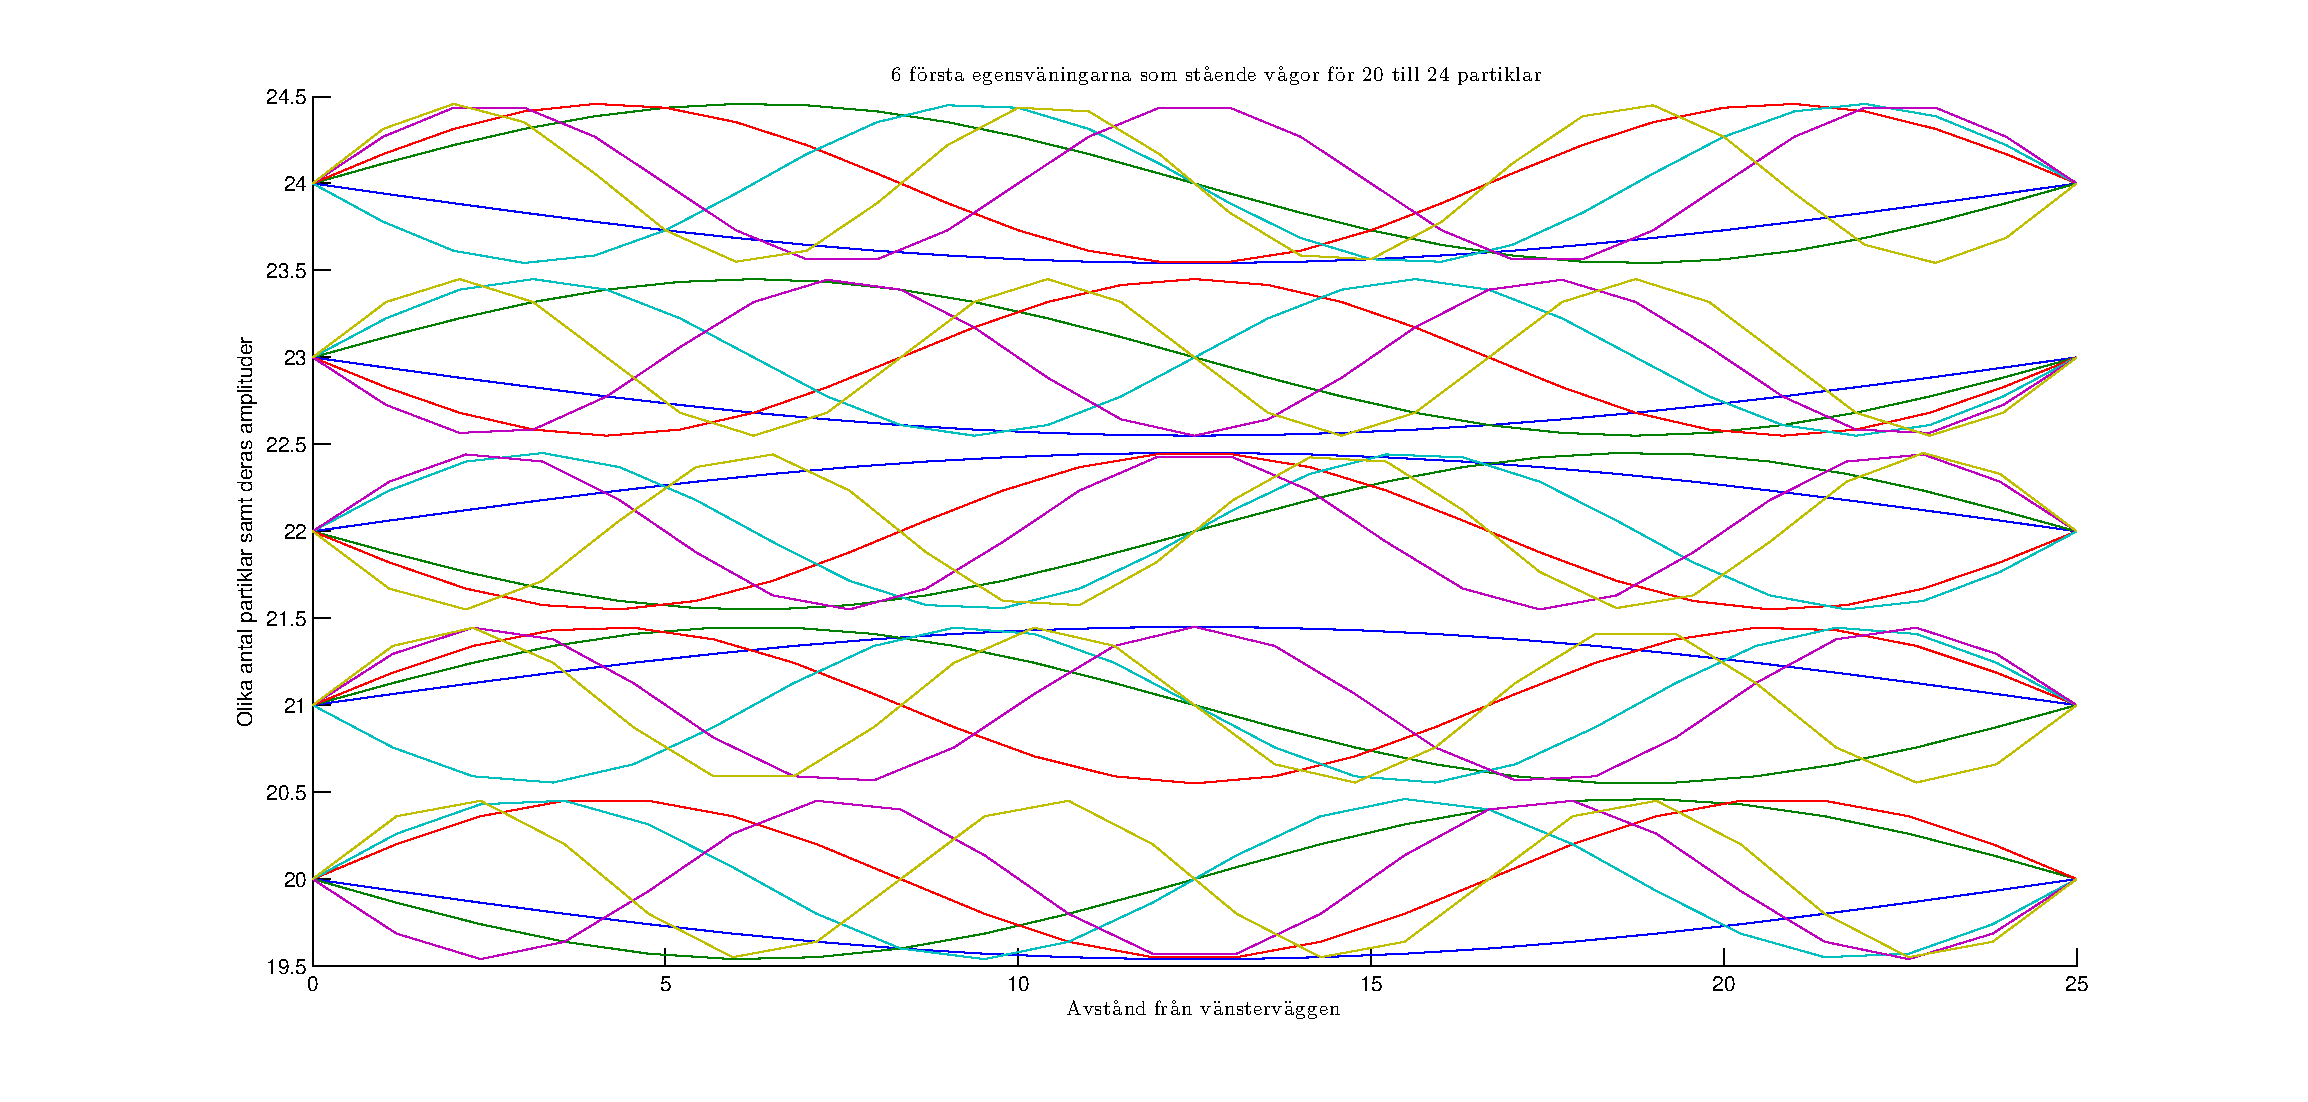
\includegraphics[width=1\textwidth]{staendevagor.eps}
			\vspace{-36pt}
			\captiona{De 6 första egensvängingarna som stående vågor. y-axeln
			för de respektive plottarna motsvarar partiklarnas avvikelse från jämnviktslägget,
			dess amplitud.}
			\label{stavag}
		\end{figure}
		
		För att illustrera egenfrekvenserna så plottar vi sinusvågor med egenfrekvenserna. Se figur \ref{egenf}.
		
		%bilder ska fixas, 10 till 20 partiklar verkar lämpligt, över 20 lär vara för svårtyt.
		
		\begin{figure}[h]
			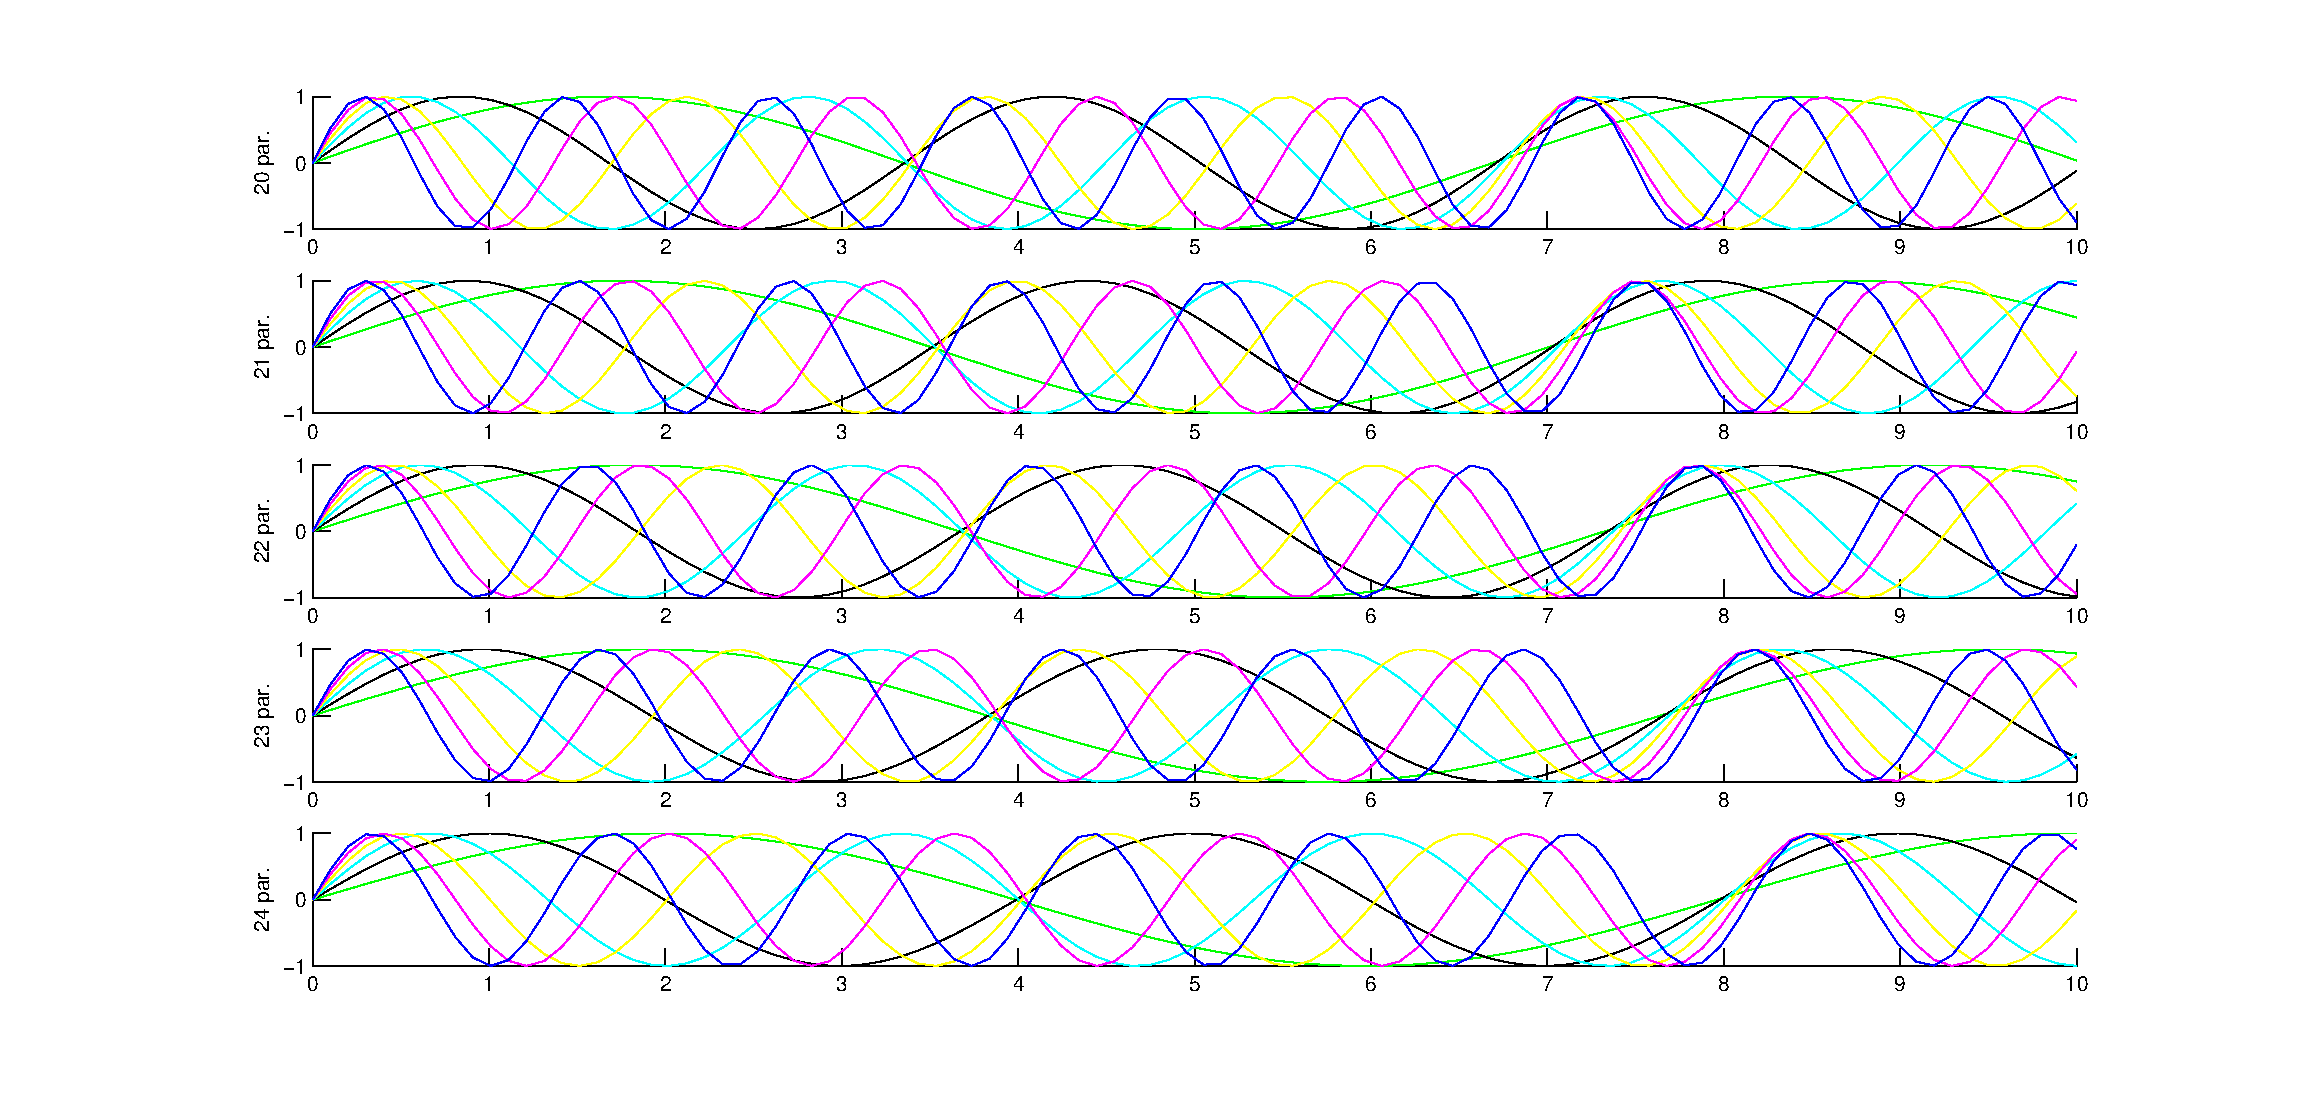
\includegraphics[width=1\textwidth]{egenfrekvenser.eps}
			\vspace{-28pt}
			\captiona{Egenfrekvenser uttryckta i $\frac{1}{\omega_o}$.}
			\label{egenf}
		\end{figure}
	
\section{Uppgift 4}
	
	\setcounter{equation}{0}
	
	\subsection{Deluppgift a}
		
		Låt $\hat{A}$ vara matrisen med de normerade egenvektorerna till den tridiagonala
		matrisen $K$, låt $\boldsymbol{\lambda}$ vara vektorn med motsvarande egenvärden samt att
		$\omega_o = k / m$ där $k$ är fjäderkonstanten och $m$ är massan hos en partikel.
		Enligt \ref{sats} kan då partiklarnas avvikelser från jämntviktsläget vid
		tiden $t$ skrivas som:
		
		\begin{equation*}
			Q(t) = \hat{A} \left[ \mathbf{C} \odot \sin(\omega_o t \sqrt{\boldsymbol{\lambda}} + \mathbf{\Phi} )\right]
		\end{equation*}
		
		där $\mathbf{C}$ och $\mathbf{\Phi}$ är vektorer med konstanter som ges av begynnelsevilkor,
		$\odot$ syftar på elementvis multiplikation (Hadamard-produkten).
		
		Med begynnelsevilkoren: 
		
		\begin{equation*}
			Q(0) = \mathbf{0} \hspace{36pt} \dot{Q}(0) = \mathbf{v}
		\end{equation*}
		
		Där $\mathbf{v}$ är en vektor för vilkoret att de mittersta $10\%$ av partiklarna ges en liten
		begynnelsehastighet, så får vi ekvationssystemet:
		
		\begin{IEEEeqnarray}{rClCrCl}
			\hat{A}\mathbf{x}       & = & \mathbf{0} & \hspace{24pt} & \mathbf{x}        & = & \mathbf{C} \odot \sin(\mathbf{\Phi})\\
			\hat{A}\dot{\mathbf{x}} & = & \mathbf{v} & \hspace{24pt} &
			\dot{\mathbf{x}}  & = & \omega_0 \mathbf{C} \odot \sqrt{\boldsymbol{\lambda}} \odot \cos(\mathbf{\Phi})
		\end{IEEEeqnarray}
		
		Då A:s kolonner är ortonormerade egenvektorer till en symmetrisk matris följer att
		$A \mathbf{x} = \mathbf{0}$ endast har trivial lösning, alltså fås ur (1) att antingen
		$\mathbf{C} = \mathbf{0}$ eller $\sin(\mathbf{\Phi}) = \mathbf{0}$. $\mathbf{C} = \mathbf{0}$ ger
		ingen lösning för (2), varpå vi får att $\sin(\mathbf{\Phi}) = \mathbf{0}$, vilket ger
		att $\Phi_i = n \pi, \,\, n \in \mathbb{N}^{\ast}$. (2) ger oss då att:
		
		\begin{equation*}
			C_i = \frac{\pm \dot{x}_i}{\sqrt{\lambda_i} \omega_o}
		\end{equation*}
		
		\begin{figure}[h]
			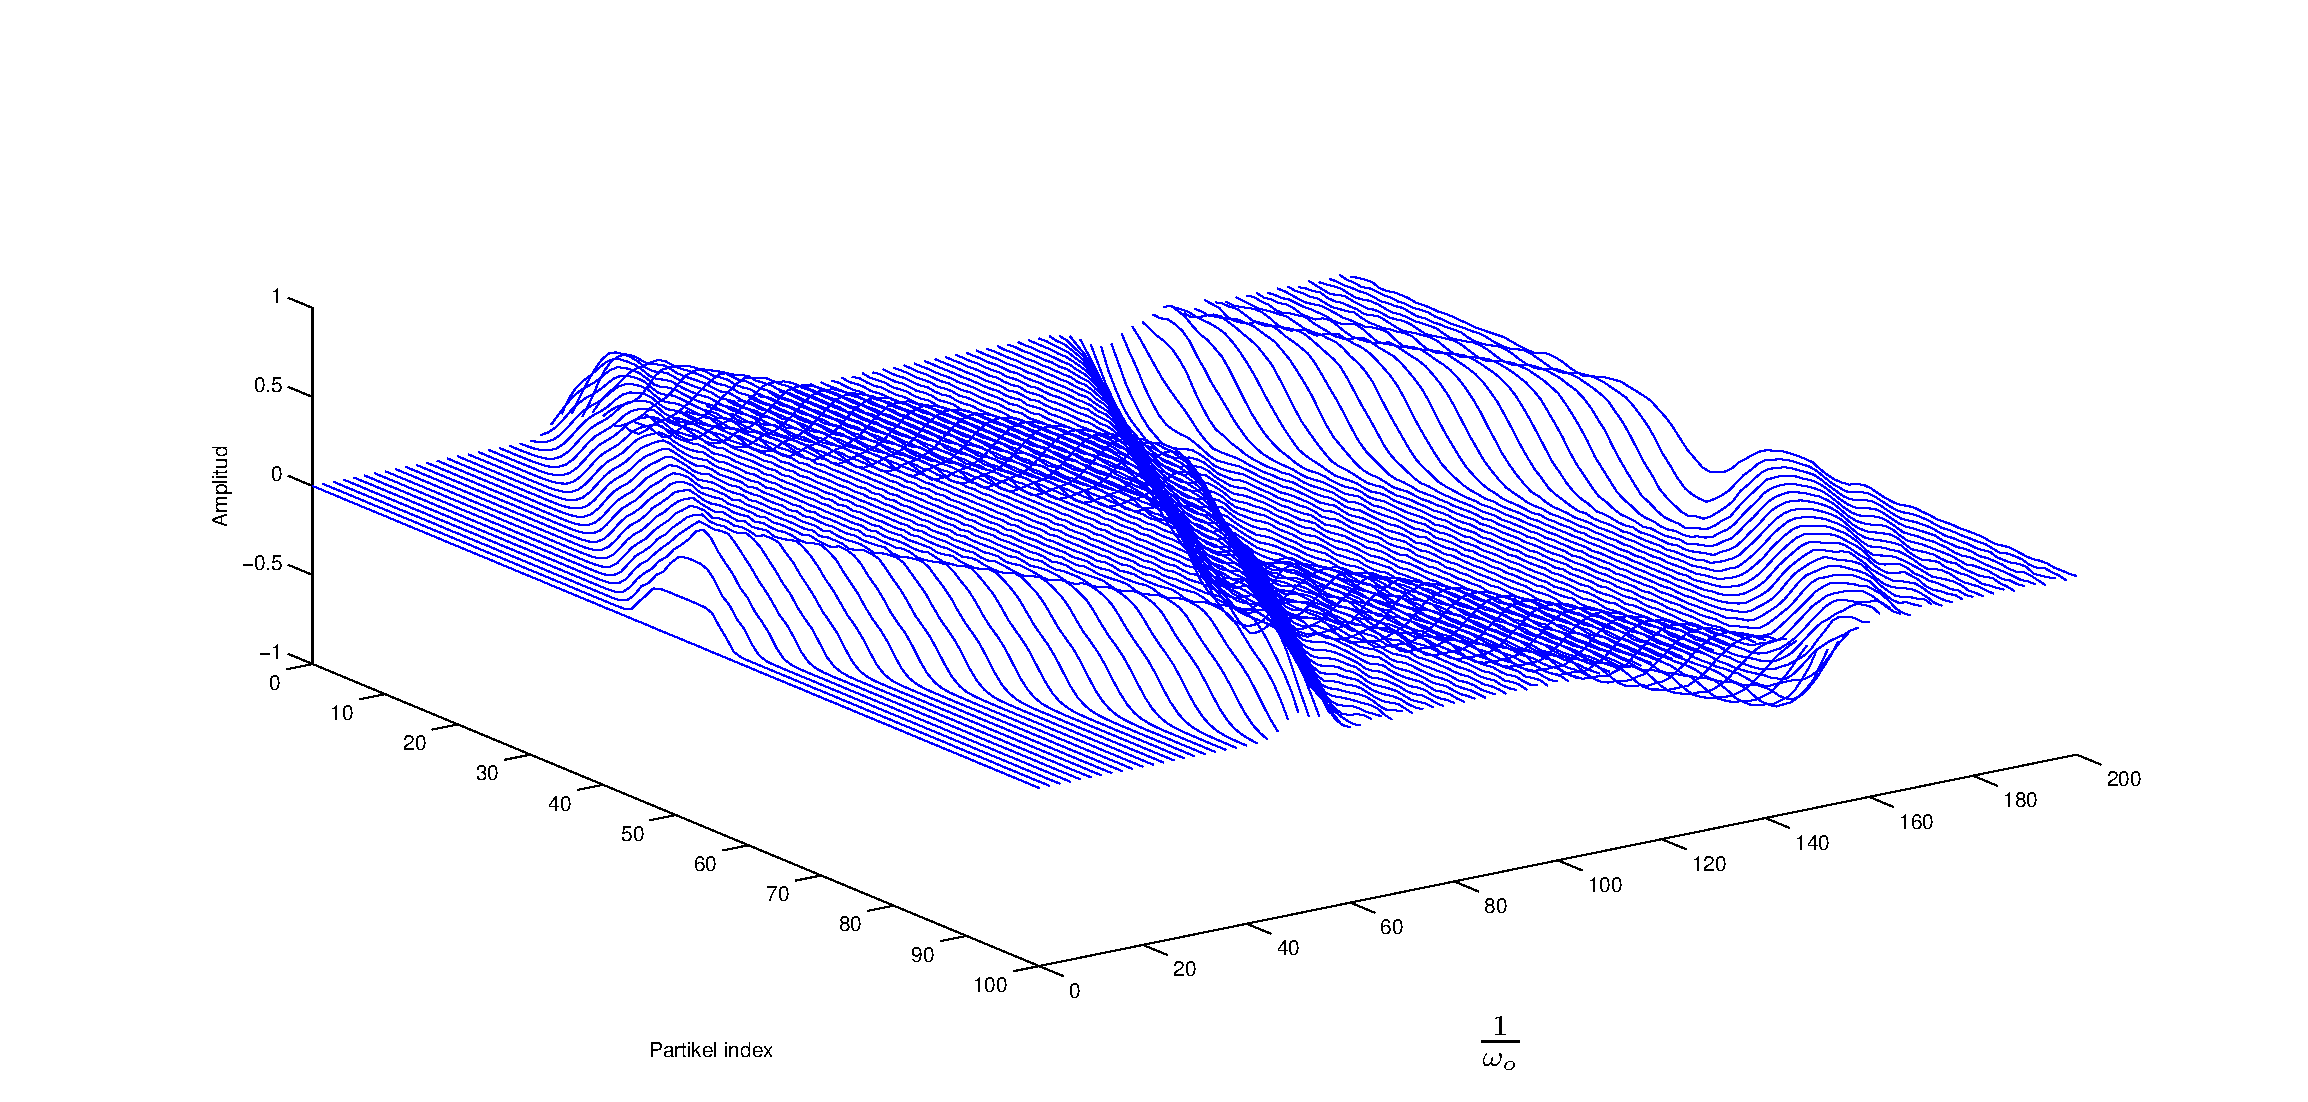
\includegraphics[width=1\textwidth]{oscillations-over-time.eps}
			\captiona{Amplitud för avvikelse hos respektive partiklar över tid, för 100 partiklar och en
			begynnelsehastighet $0.1 \, \mathrm{le} \cdot \omega_o$ för de mittersta 10 procenten av partiklarna.}
			\label{oscot}
		\end{figure}
		
		\begin{figure}[h]
			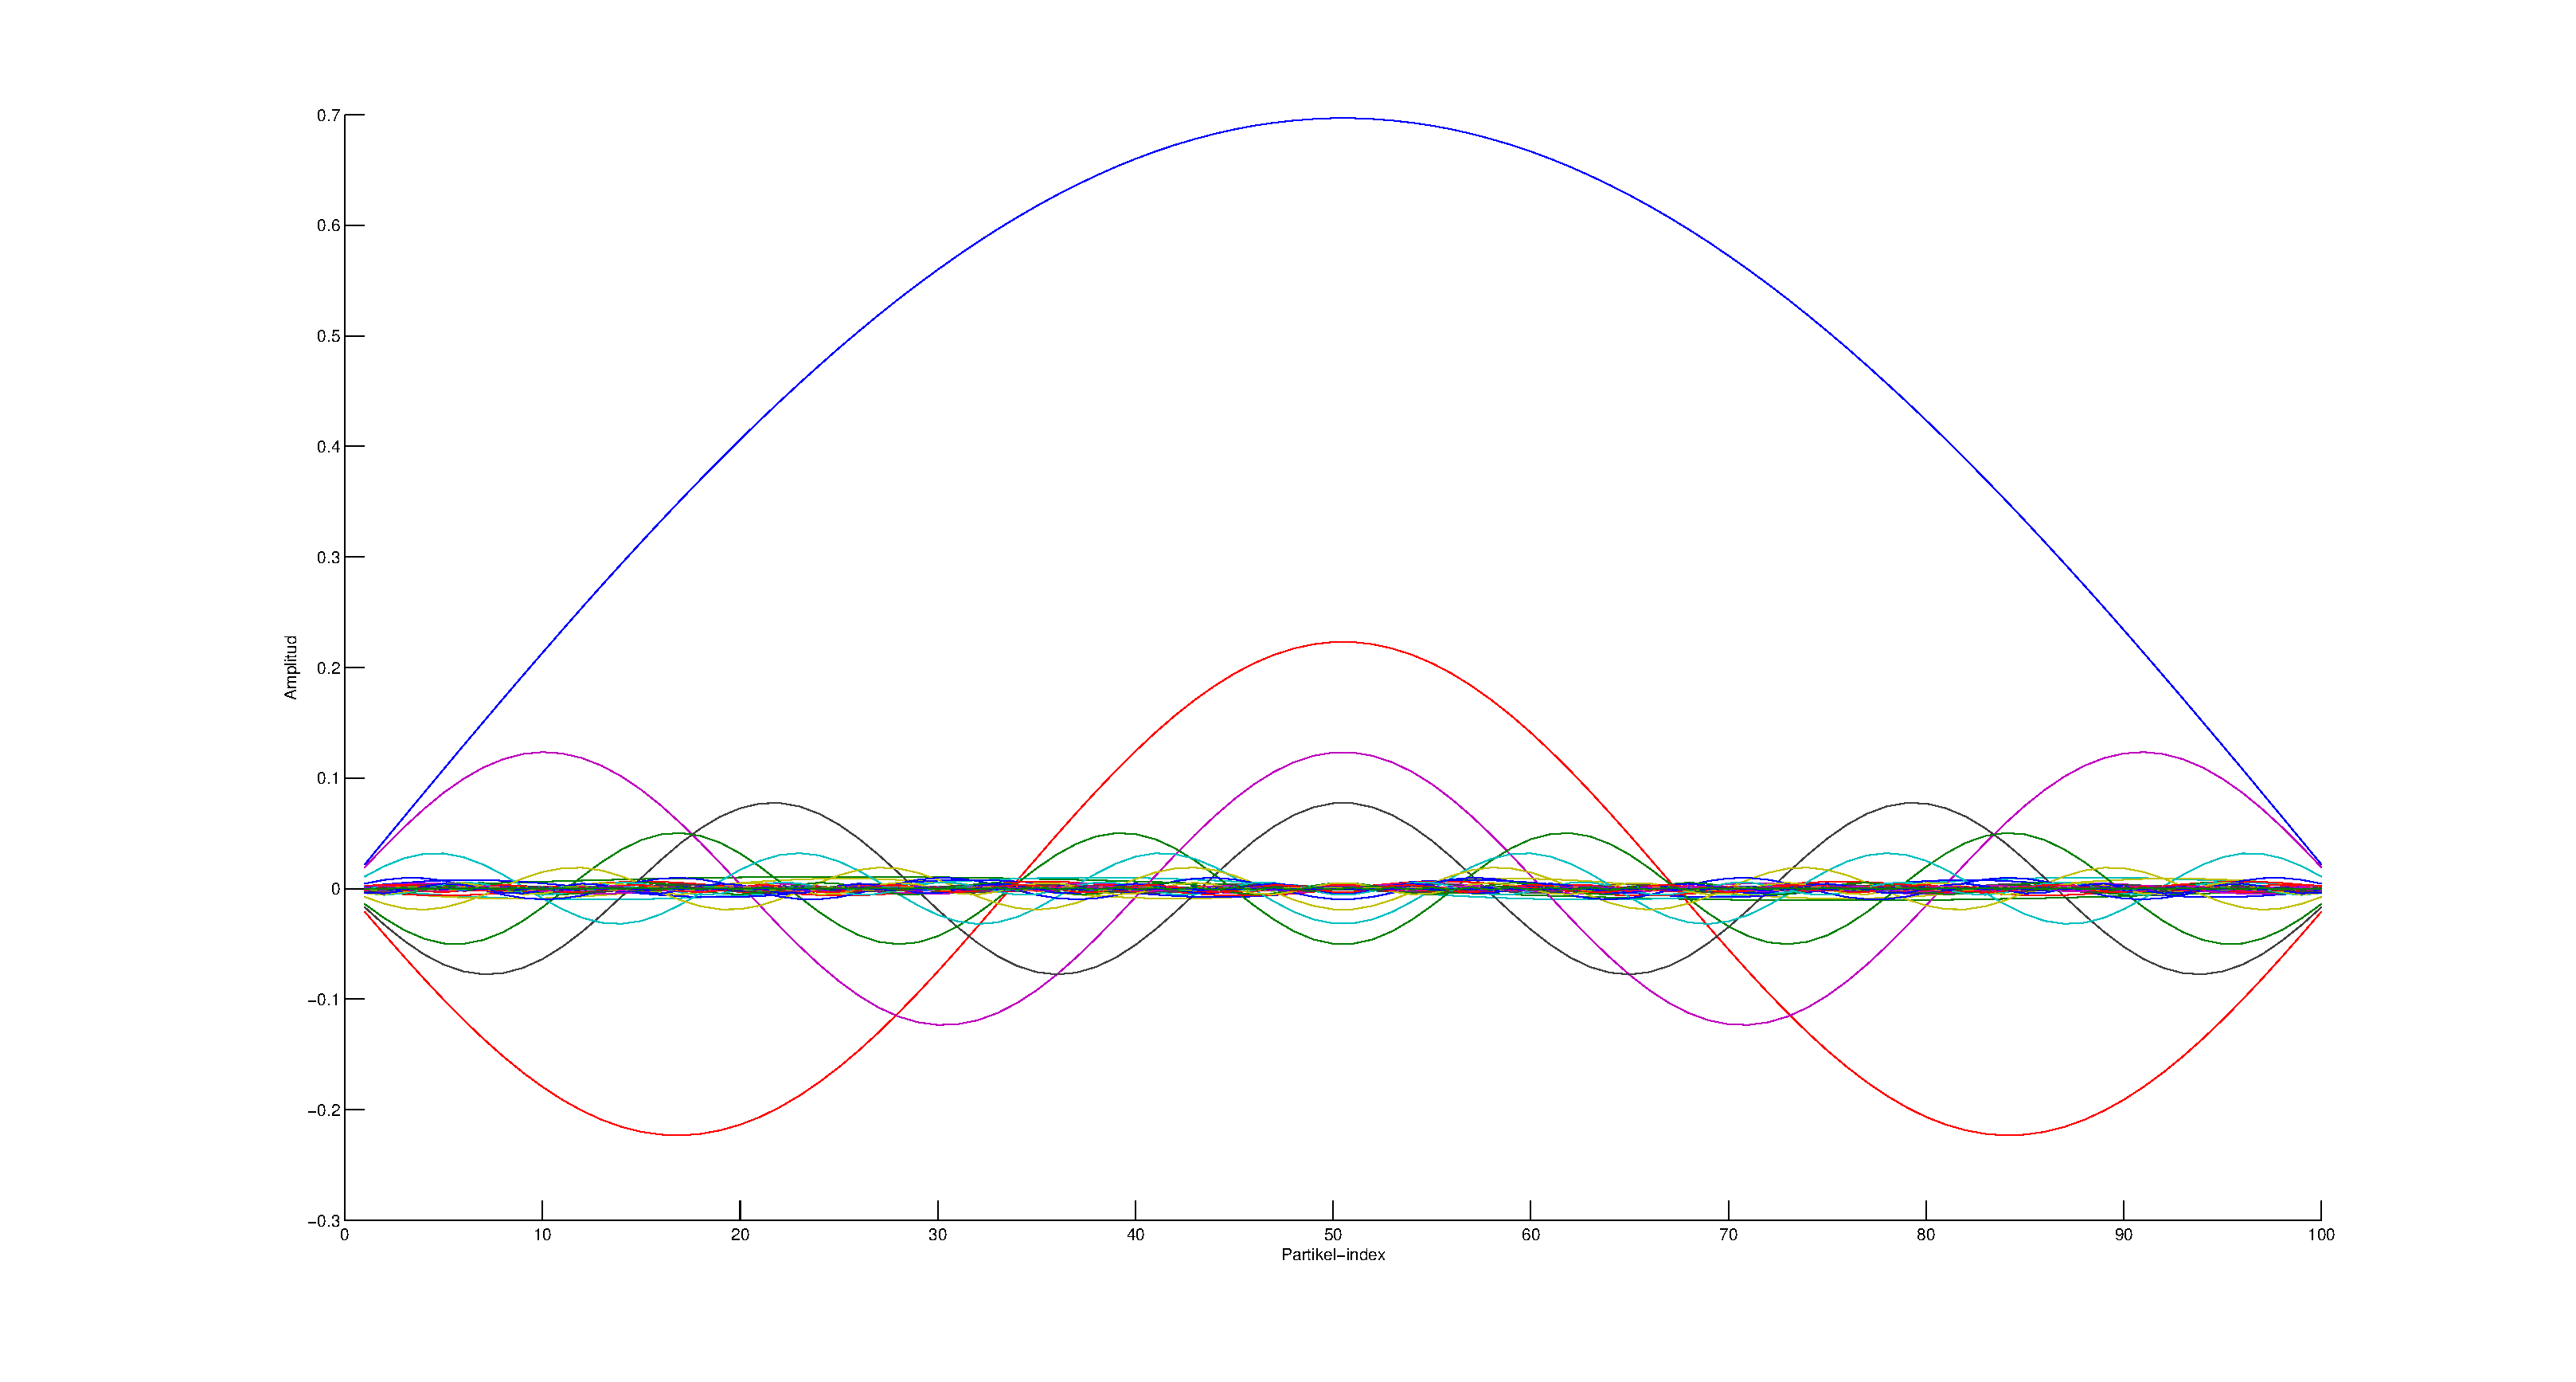
\includegraphics[width=1\textwidth]{vaagformer.eps}
			\captiona{Olika egensvängningar och deras respektive amplitud för $N=100$}
			\label{waves}
		\end{figure}
	
	\clearpage
	
	\begin{appendix}
	
		\lstset{
		  literate={ö}{{\"o}}1
		           {å}{{\aa}}1
		           {ä}{{\"a}}1
		}
		
		\lstset{language = MATLAB,
		        commentstyle = \textit,
		        showspaces = false,
		        showstringspaces = false,
		        showtabs = false,
		        tabsize = 2,
		        basicstyle = \scriptsize,
		        breaklines,
		        breakatwhitespace,
		        postbreak = \ding{229},
		        extendedchars = true
		}
		
		\section{Programkod för Uppgift 3}
			
			\begin{framed}
				\lstinputlisting[]{uppg3.m}
			\end{framed}
		
		\newpage
		
		\section{Programkod för Uppgift 4}
			
			\begin{framed}
				\lstinputlisting[]{uppg4.m}
			\end{framed}
	
	\newpage
	
\section{Sats om matrisbeskrivning av ett system av $N$ partiklar}
	
	\setcounter{equation}{0}
	
	Bevis genomfört av Torbjörn Rathsman och Martin Wernståhl.
	
	\subsection{Förutsättningar}
		\label{assumptions}
		
		\begin{itemize}
			\item Fjädrarna bevarar sin jämnvikts-längd under töjning.
			\item Alla fjädrar är linjära med fjäderkonstant $k$, deras vikt försummas.
			\item Alla partiklar räknas som punktmassor och har samma massan $m$.
			\item Observatören befinner sig i ett inertialsystem.
			\item För väggarna gäller att $q_0 = q_{N+1} = 0$, ty deras position är fix relativt observatören.
			\item $Q: \R \rightarrow \R^N,\, Q \in \mathcal{C}^2,\,Q(t) = \begin{bmatrix}q_1(t) \\ \vdots \\ q_j(t) \\ \vdots \\ q_N(t) \end{bmatrix}$ där $q_j$ är
			      partikeln $j$'s avvikelse från sitt jämnviktsläge.
			\item Varje partikel är ansluten till två fjädrar som påverkar partikeln
			      med $F = -k \Delta x$, där $\Delta x$ är fjäderns utsträckning från sin jämnviktslängd.
		\end{itemize}
	
	
	\subsection{Sats}
		\label{sats}
		
		Ett system med $N$ partiklar som uppfyller villkoren definierade i \ref{assumptions} kan skrivas
		på formen:
		
		\begin{equation*}
			\ddot{Q} + \omega_{o}^{2} K Q = 0
		\end{equation*}
		
		Där $K$ är en tri-diagonal matris med värdena $-1$, $2$, $-1$ och $\omega_o = \sqrt{\frac{k}{m}}$.
		
	\newpage
	
	\subsection{Bevis}
	\subsubsection*{$N=1$:}
		
		Enligt friläggning:
		
		\begin{equation*}
			\ddot{q_1} = \frac{-2 k q_1}{m} \hspace{12pt} \Leftrightarrow \hspace{12pt} \ddot{Q} + \omega_o^2 \begin{bmatrix}2\end{bmatrix} Q = 0
			\label{N=1}
		\end{equation*}
		
		Där då $\begin{bmatrix}2\end{bmatrix}$ är vår sökta matris $K$ enligt \ref{sats}.
		
	\subsubsection*{$N=2$:}
		
		Enligt friläggning:
		
		\begin{equation*}
			\left\{ \,
			\begin{IEEEeqnarraybox}[\IEEEeqnarraystrutmode][c]{rCl}
				\ddot{q_1} & = & -\frac{k q_1}{m} - \frac{k(q_1-q_2)}{m} \\
				\ddot{q_2} & = & -\frac{k q_2}{m} - \frac{k(q_2-q_1)}{m}
			\end{IEEEeqnarraybox}
			\right.
			\hspace{12pt}
			\Leftrightarrow
			\hspace{12pt}
			\ddot{Q} + \omega_o^2 \begin{bmatrix}
				2 & -1 \\
				-1 & 2
			\end{bmatrix} Q = 0
			\label{N=2}
		\end{equation*}
		
		Där då $\begin{bmatrix}
			2 & -1 \\
			-1 & 2
		\end{bmatrix}$ är vår sökta matris $K$ enligt \ref{sats}.
		
	\subsubsection*{$N = \{x: x \in \N \land x > 2\}$:}
		
		Antag att för $N - 2$:
		
		\begin{equation}
			q_{N-2} = -\frac{k (q_{N-2} - q_{N-3})}{m} + \frac{k(q_{N-1}-q_{N-2})}{m}
			\label{N=x 1}
		\end{equation}
		
		För partikel $N$ gäller:
		
		\begin{equation}
			q_N = -\frac{k q_N}{m} + \frac{k (q_{N-1} - q_N)}{m}
			\label{N=x N}
		\end{equation}
		
		Enligt Newton III så påverkas partikel $N - 1$ med en kraft som är lika stor
		som $k(q_{N-1} - q_{N-2}) + k (q_{N-1} - q_N)$ (följer från \ref{N=x 1} och \ref{N=x N})
		men motriktad:
		
		\begin{equation}
			q_{N-1} = -\frac{k(q_{N-1}-q_{N-2})}{m} + \frac{k (q_N - q_{N-1})}{m}
		\end{equation}
		
		Ur detta följer att:
		
		\begin{equation*}
			\begin{cases}
				q_1 = -\frac{k q_1}{m} + \frac{k(q_2 - q_1)}{m} \\
				\hspace{64pt} \vdots \\
				q_j = -\frac{k (q_j - q_{j-1})}{m} + \frac{k(q_{j+1}-q_j)}{m} \\
				\hspace{64pt} \vdots \\
				q_N = -\frac{k q_N}{m} + \frac{k (q_N - q_{N-1})}{m}
			\end{cases}
		\end{equation*}
		
		Vilket motsvarar:
		
		\begin{equation*}
			\ddot{Q} + \omega_o^2 \begin{bmatrix}
				2 & -1 & 0 & & \cdots & 0 \\
				-1 & 2 & -1 & 0 & \cdots & \\
				0 & \ddots & \ddots & \ddots & & \vdots \\
				\vdots &  & \ddots & \ddots & \ddots & 0 \\
				& \cdots & 0 & -1 & 2  & -1 \\
				0 & \cdots & & 0 & -1 & 2
			\end{bmatrix} Q = 0
		\end{equation*}
		
		där då vårt sökta $K$ från \ref{sats} är en tridiagonal matris med värdena $-1$, $2$, $-1$.
		
		Enligt Induktionsaxiomet stämmer då \ref{sats} för alla $N \geq 1$ \hfill $\square$
		
	\end{appendix}
\end{document}
